\scanpage{24}
\usetikzlibrary{shapes.geometric}
% Upright layer, from the upper edge downwards. Several diagonal cancellations
% intersect writing in a second orientation; their extent is uncertain.
\[G=\unsure{\operatorname{Aff}|\operatorname{GP}}(\unsure{G_a|\mathfrak g})\]
\[
\deleted{\operatorname{Hom}_{\unsure{k'\text{-alg}|k'\otimes_k k'}}(\unsure{k'},G)=G'}
\]
\diagram{\begin{tikzcd}[ampersand replacement=\&]
\deleted{G}\arrow[r]\&\deleted{G'}\arrow[r]\&{}\&\deleted{\unsure{\mathscr L|\mathcal L}}
\end{tikzcd}}
\deleted{\uline{\unsure{ss-grpe} \unsure{invariant}}}
\[\deleted{R_1\subset G_1}\qquad\unsure{\mathfrak h|h}\]
\diagram{\begin{tikzcd}[ampersand replacement=\&,row sep=small]
k_0(t^{\unsure{1/p|1/q}})\arrow[d,dash]\\
k_0(t)
\end{tikzcd}}
\[\unsure{h_1|k_1}\]
\diagram{\begin{tikzcd}[ampersand replacement=\&,column sep=large]
{}\arrow[rr,leftrightarrow,bend left=20]\&\deleted{\unsure{\mathfrak g|\mathscr G}}\ G\&{}
\end{tikzcd}}
\diagram{\begin{tikzcd}[ampersand replacement=\&]
\deleted{G}\arrow[r,bend left=10]\&\deleted{G'}\arrow[l,bend left=35,"\deleted{\unsure{\operatorname{Norm}_{k'/k}}}"']\&R'\&\deleted{B}
\end{tikzcd}}
\[G\qquad\mathfrak g\quad\unsure{\mathfrak h|h}\qquad H^1\]
\[\boxed{\deleted{\mathfrak g\quad\mathfrak g}}\]
% The unlabelled double-cone/hourglass drawing between the two boxed equalities.
\figure{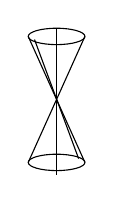
\begin{tikzpicture}[x=0.8cm,y=0.8cm]
\draw (0,2) ellipse (0.45 and 0.13);
\draw (-0.45,2)--(0.45,0) (0.45,2)--(-0.45,0);
\draw (0,0) ellipse (0.45 and 0.13);
\draw (0,2.13)--(0,-0.2);
\draw (-0.35,1.95)--(0.35,0.06);
\end{tikzpicture}}
\diagram{\begin{tikzcd}[ampersand replacement=\&]
\deleted{\mathscr L,=\mathscr L'}\&
\boxed{\deleted{[B_0=B'_0]\quad B,B'\supset T}}\arrow[d,Rightarrow,"?"']\\
{}\&\deleted{\unsure{B|R}=B'}
\end{tikzcd}}
\noindent En car $\ne\text{\uuline{$2,3,5$}}$

O.K.
\[\boxed{\deleted{\mathscr L=\mathscr L'}}\qquad\deleted{\unsure{R|B}}\]
\[H^1(B,\mathscr L)\]

% Left-edge layer, read clockwise through 90 degrees. Shared labels occur once.
% margin note written sideways; its arrows connect to the adjacent statements.
\diagram{\begin{tikzcd}[ampersand replacement=\&,column sep=small,row sep=large]
{}\&\begin{gathered}\text{Radical \inserted{\mbox{\tikz[baseline=(c.base)]{\node[draw,ellipse,inner sep=1pt] (c) {\unsure{géométrique|géométr.}};}}} défini sur }k,\\
\text{pour tt \unsure{grpe} sur tt corps }k\end{gathered}\\
\deleted{\unsure{H^1(B,\mathfrak g/\mathfrak b)=0}}\arrow[r,Rightarrow,bend left=15]\&
\begin{gathered}\text{Une \uline{variation infinitésimale}}\quad\inserted{\mbox{\tikz[baseline=(c.base)]{\node[draw,ellipse,inner sep=1pt] (c) {$\unsure{k'/k|\bar k/k}$};}}}\\
\text{d'un \uline{Borel} est \uline{triviale}}\\
\text{(i.e. }\unsure{\bar k|k'}\text{\unsure{-conjugué})}\end{gathered}\arrow[u,Rightarrow]\arrow[d,Leftrightarrow]\\
\unsure{H^1(\mathfrak u,\mathfrak u)^{T}=0|H^1(u,u)^T=0}\arrow[u,Rightarrow]\&
\begin{gathered}\text{\uline{Une telle variation}, avec un tore maximal fixé,}\\
G\text{ est \uline{constant}.}\end{gathered}
\end{tikzcd}}
% margin note written sideways; upper part of the narrow inner column
\margin{($R$ radical \uline{\unsure{unip.}}) \illegible{2}}
\[
H^1(R,\deleted{\unsure{\mathfrak g}}\mathfrak g/\mathscr L)^{B/R}=0
\]
\diagram{\begin{tikzcd}[ampersand replacement=\&,column sep=small]
{}\arrow[r]\&\deleted{H^1(B',\mathfrak g/\mathscr L)}\arrow[r]\&
\deleted{H^1(B,\mathfrak g/\mathscr L)}\arrow[r]\&
\deleted{\underline{H^1(\unsure{k'/k|k'},\mathfrak g/\mathscr L)^{B'}}}
\end{tikzcd}}
% Right-edge note, also read clockwise.
% margin note written sideways
\margin{Ça se déforme dans $G.\mathfrak g$ \deleted{$\operatorname{SL}(2).\unsure{\mathfrak{sl}(2)|\operatorname{sl}(2)}$} pour $G=\operatorname{SL}(2)$ (\uline{$\unsure{H_e|H}$} \unsure{anti-algèbre|cohomologique|pathologique}).}
% Lower-right boxed note, read clockwise. The end is crossed by an arrow.
% margin note written sideways
\margin{\fbox{\parbox{1.8cm}{il suffit que les \unsure{caractères} de $T$ \unsure{intervenant|intervenants} dans $\mathfrak g/\mathscr L$ n'interviennent pas \unsure{dans} \illegible{1}}}}
% Isolated broad arrow at the bottom-left corner.
\figure{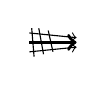
\begin{tikzpicture}[x=0.3cm,y=0.3cm]
\draw[->,line width=1.2pt] (0,0)--(2,0);
\draw[->] (0,0.4)--(2,0.2);
\draw[->] (0,-0.4)--(2,-0.2);
\draw (0.2,-0.6)--(0.1,0.6) (0.6,-0.5)--(0.4,0.6) (1,-0.4)--(0.8,0.5);
\end{tikzpicture}}
% archive sheet number: 23
